\begin{frame}{FAIR session with AuBi}


\begin{frame}
\includegraphics[page=13,scale=0.6]{01_OS_and_FAIR_intro.pdf}
\end{frame}

\begin{block}{Objectives}<1->
\begin{itemize}
\item Discover FAIR practices
\item Discover tools for best practices
\item Use tool and best practices in practice sessions
\item 5 sessions for courses and practices
	\begin{itemize}
	\item Day 1: Introduction to FAIR training and Git
	\item Day 2: Git practice
	\item Day 3: Encapsulation course
	\item Day 4: Encapsulation training
	\item Day 5: Documentation course and training
	\end{itemize}
\end{itemize}
\end{block}
\end{frame}
\section{Training content}
\begin{frame}
\begin{block}{Contents}
\begin{itemize}
\item<1-> Introduction to FAIR practices
\item<2-> Code control using Git \faGit* 
	\begin{itemize}[<2->]
	\item Git environment
	\item Gitlab and Github \faGithub \faGitlab
	\end{itemize}
\item<3-> Encapsulation process
	\begin{itemize}[<3->]
	\item Conda environment and packages use 
\includegraphics[scale=0.07]{images/conda_logo.pdf}
	\item Containers as docker \& singularity \faDocker 
	\item Reproducible workflow using snakemake 	
\includegraphics[scale=0.05]{images/snakemake_logo.png}
	\end{itemize}
\item<4-> Literate programming and documentation
	\begin{itemize}[<4->]
	\item Markdown syntax \faMarkdown
	\item Rmarkdown for R \faRProject 
	\item Jupyterlab for Python \faPython
	\end{itemize}
\end{itemize}
\end{block}
\end{frame}

